\documentclass{article}
\usepackage[utf8]{inputenc}
\usepackage{bussproofs}
\title{ProgettoLC parte5parz Gruppo 2 Relazione}
\author{Gruppo 2 }

\usepackage{tikz}
\usetikzlibrary{arrows.meta,positioning,matrix}

\usepackage{listings}
\usepackage{graphicx}
\usepackage{pdfpages}

\usepackage{hyperref}

\usepackage{imakeidx}
\makeindex

\begin{document}

\pagenumbering{gobble}
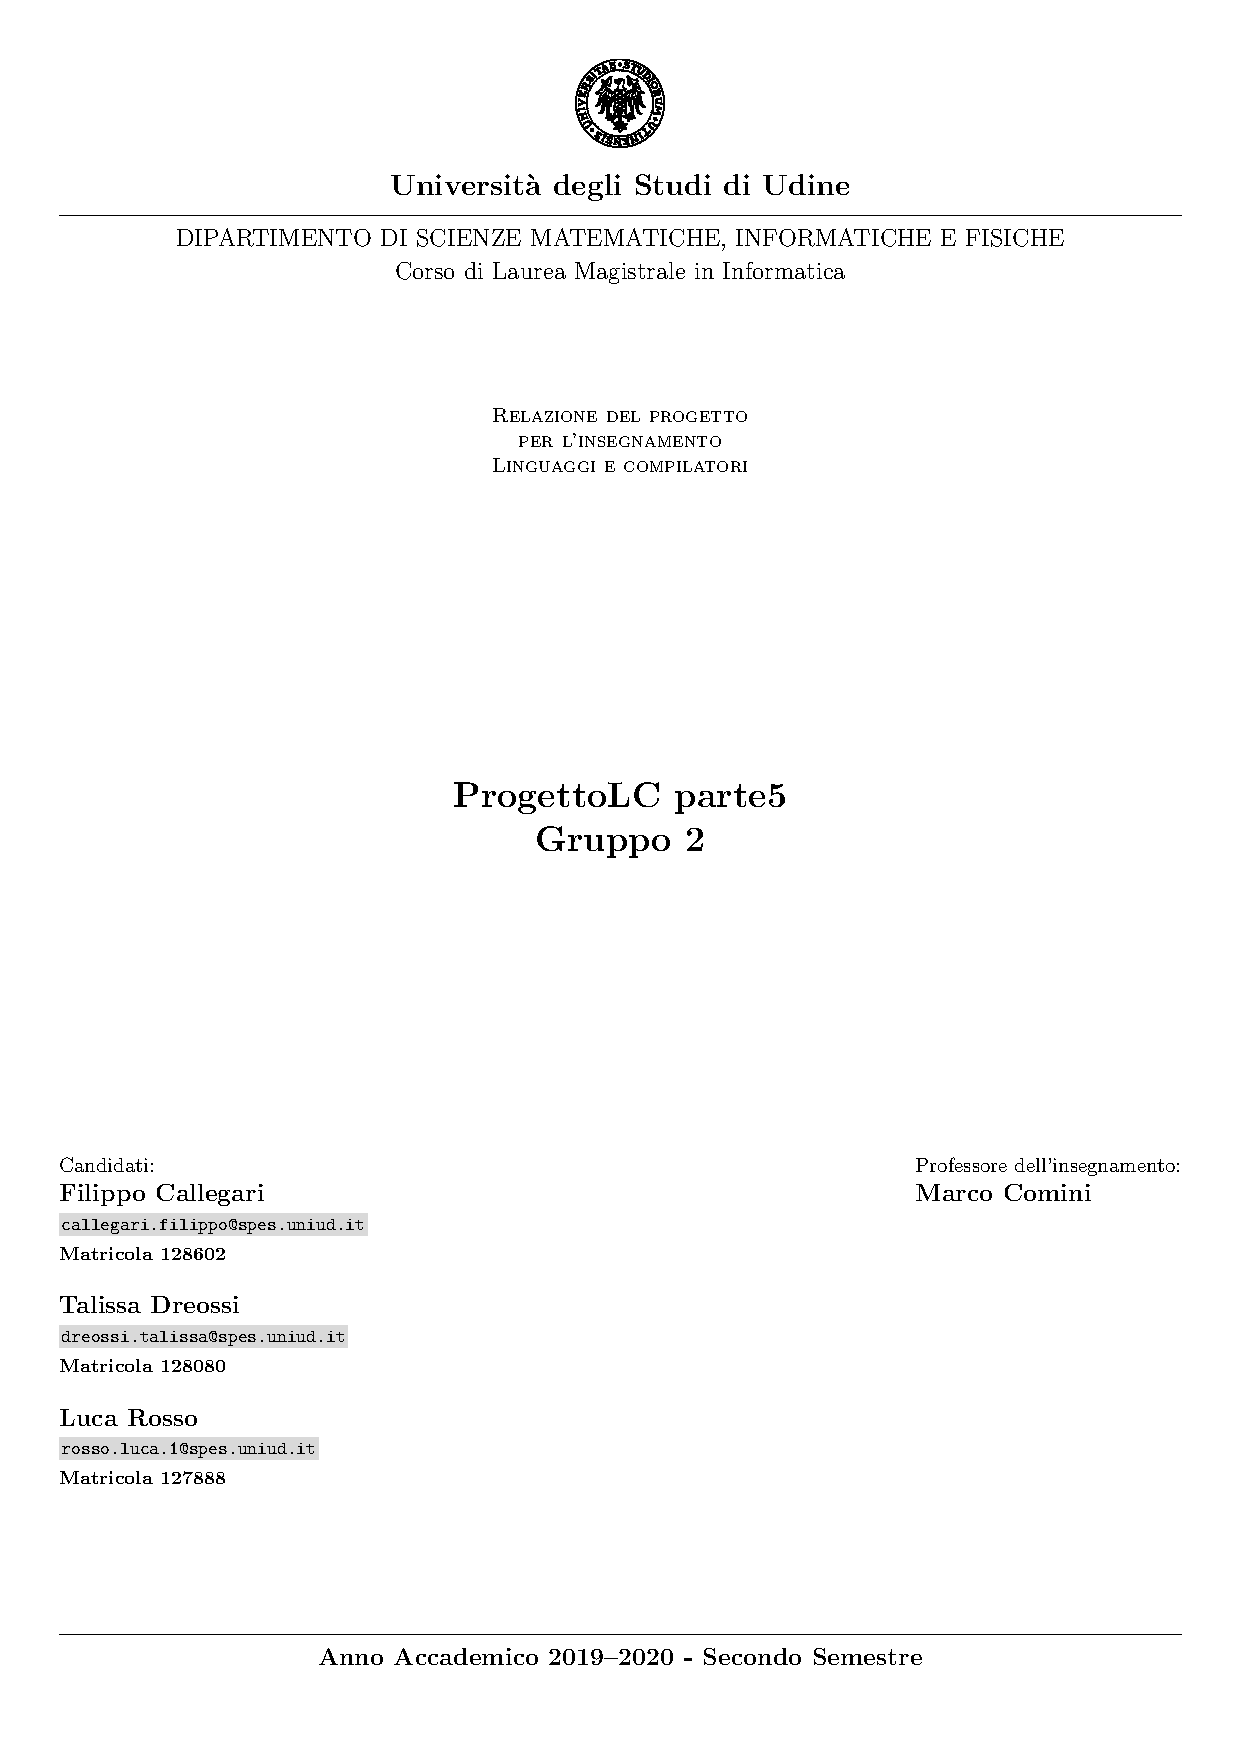
\includepdf[pages={1}]{testa.pdf}

\printindex


\pagenumbering{arabic}
\setcounter{page}{1}

\section{Scelte implementative}
L'implementazione del auL, seppur semplice, denota alcune particolarità, dovuta, tra le altre cose, a voler utilizzare
meno attributi possibili in Happy, e di creare un linguaggio solido.

La valutazione della dereferenziazione viene effettuata leggendo la parte di AST creata, dando precedenza all'array
e successivamente al puntatore, in quanto il tipo complesso (ad esempio, *Int[]) viene memorizzato come array di
puntatori.

Viene creato e manipolato passo-passo un SDT: questo permette di creare sia l'AST che il TAC contemporaneamente.

In auL sono presenti le modalità di passaggio dei parametri by value (val), by constant (const), by 
result (res) and by value/result (valres) e riferimento (gestito come definizione di Higher-Type). 
Se la modalità non è definita, verrà usata la modalità di default che è by reference per array e stringhe 
e by value per tutti gli altri tipi.

Un programma auL è composto da una lista di Statement e/o delle funzioni: il file per essere accettato deve contenere
almeno una delle due. All'interno del blocco delle funzioni, invece, similmente ai blocchi degli statement, non è richiesto
sia presente alcuna riga di codice.

\section{Lessico di auL}
in controllo sintattico viene lasciato completamente al compilatore. Noi abbiamo sviluppato solamente la gestione
degli errori sintattici. si definisce quindi che:
\begin{itemize}
	\item un'etichetta auL sia quindi definita come\\
		\texttt{token LIdent (letter|'\_'lower)(letter|digit|'\_')*;};
	
	\item i letterali che rappresentano valori costanti di tipo intero, floating point, carattere e stringhe 
	seguono le normali convenzioni, i letterali false e true rappresentano i booleani, \texttt{'nil'} per il valore
	dei puntatori.
\end{itemize}
\subsection*{Parole riservate}
Le parole riservate in auL sono:
\begin{verbatim}
  Bool       Char       Float       Int
  String     Void       and         break
  const      continue   do          else        
  elseif     end        false       for
  function   if         local       nil
  not        or         readChar    readFloat
  readInt    readString repeat      res
  return     then       true        until
  val        valres     while       writeChar
  writeFloat writeInt   writeString
\end{verbatim}

\subsection*{Simboli riservati}
I simboli riservati sono:
\begin{verbatim}
   *   [   ]  ;  =   {   }   ,
   (   )   ?  :  ==  ~=  <   <=
   >   >=  +  -  /   %   ^   ..
   #   &
\end{verbatim}
\subsection*{Commenti}
Sono presenti sia commenti in-line che commenti multi-line. Sono definiti quindi dalle seguenti espressioni regolari
\begin{verbatim}
-- Toss single line comments
"--" [.]* ;
-- Toss multi line comments
"--[" ("=")* "[" ([$u # [\]]])* ("]") ("=")* "]" ;
\end{verbatim}

\section{Sintassi di auL}
In auL un programma è definito come una lista non vuota di statement o funzioni.
\begin{verbatim}
  Program ::= [PGlobl] ;
  PGlobl ::= Stm ;
  PGlobl ::= FuncD ;
\end{verbatim}

Le dichiarazioni di entità dell'ambiente sono definite quindi come \texttt{Decl}, \texttt{Local}, ed in ambiente globale,
come \texttt{FuncD}:
\begin{verbatim}
  Decl ::= BasicType LExp VarInit ;

  BasicType ::= "Bool" | "Char" | "Float" 
              | "Int" | "String" | "Void" ;
  
  LExp ::= LIdent | "*" LExp | LIdent [Dim] ;

  Dim ::= "[" RExp "]" ;

  VarInit ::= {- empty -} | "=" RExp | "=" Array ;

  Array ::= "{" [Array] "}" | "{" [VType] "}" ;

-- le regole interne a VType sono valori assumibili
  VType ::= Boolean | Char | Double | Integer | String | PtrVoid;
  
  Local ::= "local" Decl;
  
  FuncD ::= CompoundType "function" LIdent "(" [ParamF] ")" Block "end";

  ParamF ::= Modality BasicType LExp;

  CompoundType ::= BasicType | "*"  CompoundType 
                 |  BasicType [Bracks] ;
  Bracks ::= "[" "]";
\end{verbatim}
Nella manipolazione della left expression, si dà priorità alla dereferenziazione come array, per essere
seguita dalla dereferenziazione per ``\texttt{*}''. Se fosse possibile operare con i puntatori, sommando
o moltiplicando, la dereferenziazione come array sarebbe zucchero sintattico per l'espressione \texttt{*(*(Ptr +i)+j)} .

Gli statement sono definiti come:
\begin{verbatim}
  Stm ::= Decl ";";
  Stm ::= Local ";";
  Stm ::= LExp "=" RExp ";";
  Stm ::= "while" RExp EBlk ;
  Stm ::= "repeat" Block "until" RExp ";";
  
  Stm ::= "for" LIdent "=" RExp "," RExp Increment EBlk ;
  Increment ::= {-empty-} | "," RExp ;
  
  Stm ::= "if" RExp "then" Block [ElseIf] Else "end" ;
  ElseIf ::={-empty-} | "elseif" RExp "then" Block ;
  Else ::={-empty-} | "else" Block;
  
  Stm ::= FuncWrite ";" | FuncRead ";" | Func ";";
  FuncWrite ::= "writeInt" "(" RExp ")"
              | "writeFloat" "(" RExp ")"
              | "writeChar" "(" RExp ")"
              | "writeString" "(" RExp ")";
  FuncRead  ::= "readInt" "(" ")"
              | "readFloat" "(" ")"
              | "readChar" "(" ")"
              | "readString" "(" ")";
  Func      ::= LIdent "(" [RExp] ")";
  
  Stm ::= EBlk ;
  EBlk ::= "do" Block "end";
  
  Stm ::= "return" RValue ";";
  Stm ::= "break" ";";
  Stm ::= "continue" ";";
  
  Block ::= [Stm];
  
  
\end{verbatim}

Per motivi di getsione dell'ambiente si è deciso di definire una regola fittizia (e quindi non presente in BNFC ma solo
in Happy) di \texttt{Block}: questa permette quindi di controllare e gestire il return nelle funzioni. Il blocco definito
all'interno di uno statement o dichiarazione di funzione è valido anche se vuoto, mentre la lista \texttt{PGlob} non sarà
mai accettata se non è presente almeno uno statement o una funzione. Lo statement di \texttt{return} diventa, quindi, 
disponibile solo all'interno di funzioni.

Il \texttt{break} ed il \texttt{continue} vengono resi disponibile all'utilizzo solo all'interno di cicli indeterminati.

Si nota quindi come non sia possibile eseguire in qualunque ambiente la sola esecuzione di una right expression, ma si
possa eseguire qualunque genere di funzione.

Il \texttt{For} ha opzionale la parte di \texttt{Increment}: nel caso in cui non sia presente si assume che l'incremento
sia di \texttt{1 : Int}.

La condizione di iterazione per il \texttt{for}
\begin{verbatim}
  for a = 1,10,2 do
    [Stm]
  end
\end{verbatim}
diventa quindi equivalente alla scrittura
\begin{verbatim}
  Int a = 1;  
  while (a < 10) do
    [Stm]
    a = a + 2;
  end
\end{verbatim}

Si dettagliano ulteriormente alcune peculiarità implementative nel capitolo omonimo.
~\\

Le right expression sono definite quindi come segue:
\begin{verbatim}
  Rexp ::= RExp ? RExp : RExp
         | RExp Op2 RExp
         | Op1 Rexp
         | FuncRead
         | Func         
         | LExp
         | ::Integer::
         | ::Float::
         | ::String::
         | ::Char::
         | nil
         | true
         | false
         | ( RExp ) ;
         
  Op2 ::= or | and
        | == | ~= | > | < | >= | <=
        | + | - | * | / | % | ^
        | .. ;
  
  Op1 ::= not
        | -
        | # ; 
\end{verbatim}

Mostriamo quindi le associatibità e le precedenze per ogni operatore.\\
Partiamo dagli operatori unari:

\begin{table}[h]
\begin{tabular}{lcr}
\hline
Operatore                                                               & Precedenza & Associatività   \\ \hline\hline
operatore condizionale (? :)                                             & 0          & non associativo \\
or                                                                      & 1          & sx              \\
and                                                                     & 2          & sx              \\
not                                                                     & 3          & sx              \\
==, $\sim$=, \textgreater{}, \textgreater{}=, \textless{}, \textless{}= & 4          & non associativo \\
+, -                                                                    & 5          & sx              \\
$*$, /, \%                                                              & 6          & sx              \\
\textasciicircum{}                                                      & 7          & dx              \\
- (unario)                                                              & 8          & sx              \\
\#                                                                      & 9          & sx              \\
\&                                                                      & 10         & sx              \\ \hline
\end{tabular}
\end{table}


\section{Scoping e binding  di auL}
Lo scoping di auL è prettamente statico, similmente a C. È possibile definire quindi sole funzioni ricorsive semplici
e non mutuamente ricorsive. Il binding del linguaggio, essendo compilato, è statico.

La visibilità dei nomi, siano queste di funzioni o di variabili, è immediatamente successivo alla loro dichiarazione 
ed a tutti i loro blocchi innestati (a meno di redifinizione nei suoi blocchi). È possibile bypassare la definizione 
di un qualunque nome attraverso lo statement \textit{local}: local infatti permette di \textbf{definire una variabile} 
riutilizzando un nome già utilizzato, anche nel medesimo blocco.

Non è possibile dichiarare funzioni innestate: quando si entra in un blocco legato ad un blocco, si perde
la possibilità di definirne.

Non è possibile definire variabili locali come costanti, ma è possibile definire parametri di funzione
come tali. 

La definizione di variabili (ed array o puntatori) permette l'inizializzazione. Unico vincolo è che durante l'inizializzazione
non è possibile autoriferirsi (a meno non ci si trovi in una situazione di utilizzo dello
statement \textit{local}). La definizione di una variabile senza conseguente inizializzazione crea un valore
generico al suo interno (undefined behaviour), ed in sè non genera un errore. Non si richiede che il valore di 
inizializzazione sia noto a \textit{compile time}.

\section{Tipi e regole di auL}
\subsection{Definizione dei tipi}
In auL abbiamo identificato i seguenti tipi di base
\begin{itemize}
    \item Int
    \item Char
    \item String
    \item Float
    \item Boolean
\end{itemize}
Inoltre c'è la possibilità di definire array di dimensione prefissata e di definire dei puntatori a tipo qualsiasi. Questi sono quindi noti come
``higher-types''.

Abbiamo anche definito il tipo Void per gestire il tipo di ritorno delle funzioni che non restituiscono alcun valore.
\subsection{Compatibiltà tra i tipi}
Definiamo come \emph{tipi canonici} i tipi $C_\tau=\{Int, Float, Bool, Char, String\}$.


Mostriamo quindi la gerarchia di tipo:\\
\begin{tikzpicture}
\matrix (m) [matrix of math nodes,
row sep=3em, column sep=3em,
text height=1.5ex,
text depth=0.25ex]{
            &            &              &                             \\
Float       &   String   &              &                             \\
            &            &              &                             \\
Int         &  Char      &  Bool        &       Void                  \\
};
\path[-{Latex[length=2.5mm, width=1.5mm]}]
(m-4-1) edge (m-2-1)
(m-4-2) edge (m-2-2);
\end{tikzpicture}
~\\
~\\

Quindi deduciamo che:
\begin{itemize}
	\item se assegniamo un \emph{Int} ad un \emph{Float}, questo sarà accettato;
	\item ogni $C_{\tau}$ accetterà ogni $C_{\tau}$;
	\item se $\tau_1$ è un \emph{higher-type} puntatore, questo accetterà un $\tau_2$ \emph{higher-type} array, a patto che
		l'``\emph{altezza}'' del puntatore sia la medesima dell'``\emph{altezza}'' e\\ $C_{\tau_1} = C_{\tau_2}$;
	\item per completezza nel manipolare il tipo canonico ``$String$'' si permette di riferire una singola lettera di questa
		come fosse un array di ``$Char$'', ma non sono consentite operazioni tra ``$Char$'' e ``$String$''\footnote{Si è deciso in
		comune accordo che la dereferenziazione di una stringa generi \textbf{comunque} un tipo ``$Char$'', in quanto non sarebbe
		altrimenti possibile operare in nessuna maniera con le stringhe, come, ad esempio, per far diventare maiuscola una stringa
		minuscola. Per togliere tale possibilità è sufficiente commentare riga 232 del file ``\textit{Env.hs}''.}.
	
\end{itemize}

\section{Type system}
\subsection{Regole per le costanti}
Sia ``$a$'' un valore per un tipo ``$\tau$". Allora
	\begin{prooftree}
		\AxiomC{$\exists a \in \{\tau:Int,\tau:Bool,\tau:Float,\tau:Char,\tau:String\}$}
		\UnaryInfC{$\Gamma \vdash_{val} a : \tau$}
	\end{prooftree}

Esemplifichiamo ulteriormente ``$a$'' un valore per un tipo ``$\tau:Bool$":
	\begin{prooftree}
		\AxiomC{$a =$ `$true$'$: \tau$}
		\AxiomC{$\tau:Bool$}
		\BinaryInfC{$\Gamma \vdash_{val} a : \tau$}
	\end{prooftree}
	\begin{prooftree}
		\AxiomC{$a =$ `$false$'$: \tau$}
		\AxiomC{$\tau:Bool$}
		\BinaryInfC{$\Gamma \vdash_{val} a : \tau$}
	\end{prooftree}
Esemplifichiamo ulteriormente ``$a$'' un valore per un tipo puntatore a ``$\tau:C_\tau$":
	\begin{prooftree}
		\AxiomC{$a = $ `$nil$'$: \tau$}
		\AxiomC{$\tau: Pointer(C_\tau)$}
		\BinaryInfC{$\Gamma \vdash_{val} a : Pointer(C_\tau)$}
	\end{prooftree}
\subsection{Regole per le Right-Expressions}
\textit{S.p.d.g.} siano $a$ e $b$ delle \emph{Right expression}. Esemplifichiamo quindi il type system per le \emph{Right Expressions}.
\begin{itemize}
	\item $\tau\in\{Int,Float\}$
	\begin{prooftree}
		\AxiomC{$\Gamma \vdash_{rexp} a : \tau$}
		\AxiomC{$ -a : \tau$}
		\BinaryInfC{$\Gamma \vdash_{rexp} - a : \tau$}
	\end{prooftree}

	\item $\tau_1,\tau_2\in\{Int,Float,Char\}$, $\tau_\diamond$ rispetta la gerarchia di tipo e\\ $\odot \in \{+,-\}$
	\begin{prooftree}
		\AxiomC{$\Gamma \vdash_{rexp} a : \tau_1$}
		\AxiomC{$\Gamma \vdash_{rexp} b : \tau_2$}
		\AxiomC{$a \odot b : \tau_\diamond$}
		\TrinaryInfC{$\Gamma \vdash_{rexp} a \odot b : \tau_\diamond$}
	\end{prooftree}

	\item $\tau_1,\tau_2\in\{Int,Float\}$, $\tau_\diamond$ rispetta la gerarchia di tipo e\\ $\odot \in \{*, \div, \hat{\mkern6mu} \}$
	\begin{prooftree}
		\AxiomC{$\Gamma \vdash_{rexp} a : \tau_1$}
		\AxiomC{$\Gamma \vdash_{rexp} b : \tau_2$}
		\AxiomC{$a \odot b : \tau_\diamond$}
		\TrinaryInfC{$\Gamma \vdash_{rexp} a \odot b : \tau_\diamond$}
	\end{prooftree}

	\item $\tau_1,\tau_2\in\{Int,Float\}$
	\begin{prooftree}
		\AxiomC{$\Gamma \vdash_{rexp} a : \tau_1$}
		\AxiomC{$\Gamma \vdash_{rexp} b : \tau_2$}
		\AxiomC{$a \% b : Int$}
		\TrinaryInfC{$\Gamma \vdash_{rexp} a \% b : Int$}
	\end{prooftree}

	\item $\tau \in \{String\}$
	\begin{prooftree}
		\AxiomC{$\Gamma \vdash_{rexp} a : \tau$}
		\AxiomC{$\Gamma \vdash_{rexp} b : \tau$}
		\AxiomC{$a .. b : String$}
		\TrinaryInfC{$\Gamma \vdash_{rexp} a .. b : String$}
	\end{prooftree}
	
	\item $\tau \in \{Int, Float, Char\}$ e $\odot \in \{\leq,\geq,<,>\}$
	\begin{prooftree}
		\AxiomC{$\Gamma \vdash_{rexp} a : \tau$}
		\AxiomC{$\Gamma \vdash_{rexp} b : \tau$}
		\AxiomC{$a \odot b : Bool$}
		\TrinaryInfC{$\Gamma \vdash_{rexp} a \odot b : Bool$}
	\end{prooftree}

	\item $\tau_1,\tau_2 = C_\tau$ e $\odot \in \{==,\not=\}$
	\begin{prooftree}
		\AxiomC{$\Gamma \vdash_{rexp} a : \tau_1$}
		\AxiomC{$\Gamma \vdash_{rexp} b : \tau_2$}
		\AxiomC{$a \odot b : Bool$}
		\TrinaryInfC{$\Gamma \vdash_{rexp} a \odot b : Bool$}
	\end{prooftree}
	
	\item dove $\tau$ è puntatore a $C_\tau$ e $\odot \in \{==,\not=\}$
	\begin{prooftree}
		\AxiomC{$\Gamma \vdash_{val} a :$ `$nil$'}
		\AxiomC{$\Gamma \vdash_{rexp} b : \tau$}
		\AxiomC{$a \odot b : Bool$}
		\TrinaryInfC{$\Gamma \vdash_{rexp} a \odot b : Bool$}
	\end{prooftree}
	
	\item  il caso riflessivo per $a$ e $b$ a quello sopra;

	\item $\tau_1, \tau_2$ sono puntatore a $C_\tau$ e $\odot \in \{==,\not=\}$
	\begin{prooftree}
		\AxiomC{$\Gamma \vdash_{rexp}a : \tau_1$}
		\AxiomC{$\Gamma \vdash_{rexp}b : \tau_2$}
		\AxiomC{$a \odot b : Bool$}
		\TrinaryInfC{$\Gamma \vdash_{rexp} a \odot b : Bool$}
	\end{prooftree}

	\item $\tau$ è puntatore a $C_\tau$
	\begin{prooftree}
		\AxiomC{$\Gamma \vdash_{rexp}a : \tau$}
		\AxiomC{$\#a : Int$}
		\BinaryInfC{$\Gamma \vdash_{rexp} \#a : Int$}
	\end{prooftree}

	\item $\odot \in \{and, or\}$
	\begin{prooftree}
		\AxiomC{$\Gamma \vdash_{rexp}a : Bool$}
		\AxiomC{$\Gamma \vdash_{rexp}b : Bool$}
		\AxiomC{$a \odot b : Bool$}
		\TrinaryInfC{$\Gamma \vdash_{rexp} a \odot b : Bool$}
	\end{prooftree}
	
	\item regola unaria del not
	\begin{prooftree}
		\AxiomC{$\Gamma \vdash_{rexp}a : Bool$}
		\AxiomC{$not~a : Bool$}
		\BinaryInfC{$\Gamma \vdash_{rexp}not~a : Bool$}
	\end{prooftree}
	
	\item siano $a_1,\dots,a_n$ espressioni, $id$ identificativo di una funzione con arietà $n$ e $\tau_\diamond\in C_\tau$
	\begin{prooftree}
		\AxiomC{$\Gamma \vdash_{rexp}a_1:\tau_1,\dots,\Gamma \vdash_{rexp}a_n:\tau_n$}
		\AxiomC{$\Gamma \vdash_{rexp}id(a_1:\tau_1 \times \dots \times a_n:\tau_n) : \tau_\diamond$}
		\BinaryInfC{$\Gamma \vdash_{rexp}id(a_1,\dots,a_n) : \tau_\diamond$}
	\end{prooftree}

	\item $id$ identificativo di una variabile, $\tau$ il suo tipo (sia higher-type che $C_\tau$)
	\begin{prooftree}
		\AxiomC{$\Gamma \vdash_{lexp}id:\tau$}
		\UnaryInfC{$\Gamma \vdash_{rexp}id : \tau$}
	\end{prooftree}

	\item $id$ identificativo di una variabile, $\tau$ il suo tipo (sia higher-type che $C_\tau$) e $*\tau$ il puntatore a $\tau$
	\begin{prooftree}
		\AxiomC{$\Gamma \vdash_{lexp}id:\tau$}
		\UnaryInfC{$\Gamma \vdash_{rexp}\&id : *\tau$}
	\end{prooftree}
	
	\item sia $\phi\in\{readInt():Int,readFloat():Float,readChar():Char,readString():String\}$ funzioni del linguaggio 
		per ricevere input dal mondo esterno, ed associamo loro il tipo di ritorno
	\begin{prooftree}
		\AxiomC{$\Gamma \vdash_{rexp}\phi():\tau$}
		\UnaryInfC{$\Gamma \vdash_{rexp}\phi() : \tau$}
	\end{prooftree}
	
	\item $val$ identificativo di un valore, $\tau$ il suo tipo (sia higher-type che $C_\tau$)
	\begin{prooftree}
		\AxiomC{$\Gamma \vdash_{val}val:\tau$}
		\UnaryInfC{$\Gamma \vdash_{rexp}val : \tau$}
	\end{prooftree}
	
	\item sia $c$ un ulteriore \textit{R. Exp.}. Allora, definito l'operatore condizionale si avrà:
	\begin{prooftree}
		\AxiomC{$\Gamma \vdash_{rexp}a : Bool$}
		\AxiomC{$\Gamma \vdash_{rexp}b : \tau$}
		\AxiomC{$\Gamma \vdash_{rexp}c : \tau$}
		\TrinaryInfC{$\Gamma \vdash_{rexp} a$ \texttt{?} $b$ \texttt{:} $c : \tau$}
	\end{prooftree}
\end{itemize}
\subsection{Regole per le Left-Expression}
\textit{S.p.d.g.} sia $a$ una Left Expression. Esemplifichiamo il type system per le Left Expression.

\begin{itemize}	
	\item sia $*\tau : Pointer(C_\tau)$
	\begin{prooftree}
		\AxiomC{$\Gamma\vdash_{lexp} a : *\tau$}
		\UnaryInfC{$\Gamma \vdash_{lexp} *a : \tau$}
	\end{prooftree}
	
	\item sia $\tau[~] : Array(C_\tau)$, e sia $E \dashv_{rexp} \Gamma : Int$
	\begin{prooftree}
		\AxiomC{$\Gamma\vdash_{lexp} a : \tau[~]$}
		\AxiomC{$\Gamma\vdash_{rexp} E : Int$}
		\BinaryInfC{$\Gamma \vdash_{lexp} a[E] : \tau$}
	\end{prooftree}
	\item sia $*\tau : Poiter(C_\tau)$, e sia $E \dashv_{rexp} \Gamma : Int$
	\begin{prooftree}
		\AxiomC{$\Gamma\vdash_{lexp} a : *\tau$}
		\AxiomC{$\Gamma\vdash_{rexp} E : Int$}
		\BinaryInfC{$\Gamma \vdash_{lexp} a[E] : \tau$}
	\end{prooftree}
\end{itemize}
\subsection{Regole per la definizione di funzioni}
\textit{S.p.d.g.} sia $C$ un insieme (anche vuoto) di Statement. Esemplifichiamo il type system per la definizione di funzioni.
\begin{itemize}
	\item sia $\tau\in\{HT(C_\tau), C_\tau \cup \{Void\}\}$, $\Gamma$ l'\emph{Environment} e $\hat{\Gamma}$ l'\emph{environment} nuovo
	\begin{prooftree}
		\AxiomC{$\Gamma, id\vdash \emptyset :\perp$\footnote{~}} 
		\AxiomC{$\Gamma \vdash_{cmd} C:Void$}
		\BinaryInfC{$\Gamma \vdash_{fnct} id(a_1:\tau_1,\dots,a_n:\tau_n)\{C\} : \tau \Rightarrow (\Gamma,id(a_1:\tau_1 \times a_n:\tau_n):\tau)\models\hat{\Gamma}$ }
	\end{prooftree}
	\begin{prooftree}
		\AxiomC{$\Gamma, id\vdash \emptyset :\perp$}
		\AxiomC{$\Gamma \vdash_{cmd} C:Void$}
		\BinaryInfC{$\Gamma \vdash_{fnct} id(~)\{C\} : \tau \Rightarrow (\Gamma,id(~):\tau)\models\hat{\Gamma}$ }
	\end{prooftree}
	\begin{enumerate}
	\setcounter{enumi}{1}
	\item con ``$\Gamma, id\vdash \emptyset :\perp$'' si indica che non è mai stata definita nessuna funzione o variabile con nome definito in ``id''.
	\end{enumerate}
\end{itemize}
\subsection{Regole per la definizione di variabili}
\textit{S.p.d.g.} sia $\Gamma$ l'\emph{Environment} e $\hat{\Gamma}$ l'\emph{environment} nuovo.
Esemplifichiamo il type system per la definizione di funzioni.
\begin{itemize}
	\item sia $\tau\in\{HT(C_\tau), C_\tau\}$
	\begin{prooftree}
		\AxiomC{$\Gamma, id\vdash \emptyset :\perp$}
		\UnaryInfC{$\Gamma \vdash_{var} id : \tau \Rightarrow (\Gamma,id:\tau)\models\hat{\Gamma}$ }
	\end{prooftree}
	\begin{prooftree}
		\AxiomC{$\Gamma, id\vdash \emptyset :\perp$} 
		\AxiomC{$\Gamma \vdash_{rexp} b : Int$}
		\BinaryInfC{$\Gamma \vdash_{var} id[b] : \tau \Rightarrow (\Gamma,id:\tau)\models\hat{\Gamma}$ }
	\end{prooftree}	
	
	\item sia $\tau\in\{Pointer(C_\tau), C_\tau\}$
	\begin{prooftree}
		\AxiomC{$\Gamma, id\vdash \emptyset :\perp$} 
		\AxiomC{$\Gamma \vdash_{rexp} E :\tau$}
		\BinaryInfC{$\Gamma \vdash_{var} id = E : \tau \Rightarrow (\Gamma,id:\tau)\models\hat{\Gamma}$ }
	\end{prooftree}
	
	\item sia $\tau : HT(C_\tau)$
	\begin{prooftree}
		\AxiomC{$\Gamma \vdash_{val} a_i :\tau , \forall i \in [1,n]$}
		\AxiomC{$\Gamma \vdash_{val} E=\{a_1:\tau \times \dots \times a_n:\tau\} : \tau $}
		\BinaryInfC{$\Gamma \vdash_{val} E : \tau$}
		\AxiomC{$\Gamma, id\vdash \emptyset :\perp$} 
		\AxiomC{$\Gamma \vdash_{rexp} b : Int$}
		\TrinaryInfC{$\Gamma \vdash_{var} id[b] = E : \tau \Rightarrow (\Gamma,id:\tau)\models\hat{\Gamma}$ }
	\end{prooftree}
\end{itemize}

\subsection{Regole per i comandi}
\emph{S.p.d.g.}, per tutti i comandi appartenenti a ``\textit{auL}'', possiamo affermare che il tipo che ritorna sia sempre e solo indefinito.
\begin{prooftree}
	\AxiomC{}
	\UnaryInfC{$\Gamma\vdash_{cmd}C:\perp$}
\end{prooftree}
\section{Altri vincoli del auL}
\begin{itemize}
	\item Una chiamata di funzione in una espressione non può avere tipo di
		ritorno void, perché le espressioni non possono avere tipo void;
	
	\item \textbf{break} e \textbf{continue} possono comparire solo nel corpo di un loop indeterminato.
		In caso di loop annidati, questi statement si riferiscono al ciclo più interno;
	
	\item poichè il return è prerogativa nelle sole funzioni, e non è possibile verificare che
		venga eseguito ogni return dichiarato nei blocchi (come ``\textit{if-then-elseif-else}'',
		si è deciso che sia sufficiente lasciare che c'è almeno un blocco che lo contiene perchè
		la funzione di tipo non-\textit{Void} abbia il return richiesto. Rimane a carico del programmatore
		garantirne il corretto funzionamento;

	\item nel caso in cui il tipo della funzione sia definito come \textit{Void}, si controlla solo che
		il \textit{return} non ritorni effettivamente nulla. Oltre questo, viene considerato valido se
		in questo genere di funzioni non compaia il return.
	
	\item viene controllato, ad ogni chiamata di funzione, che il numero di parametri
		attuali coincida con il numero di parametri formali, e che i tipi
		siano compatibili;
		
	\item non è possibile sovrascrivere una costante, perciò negli assegnamenti
		si controlla che la lhs non sia una costante;
	
	\item sono implementati i passaggi per riverimento, valore, risultato, costante, valore/risultato.
		Il passaggio per valore è definibile attraverso alla dichiarazione dei parametri di funzione
		del valore in ingresso come puntatore (e quindi ``*''). I vincoli sulle ``modalità'' del parametro
		sono che se la variabile è definita come \texttt{costante} non sarà possibile modificare il suo
		valore, mentre se la variabile è in modalità ``risultato'' non sarà possibile accedere al suo valore.
\end{itemize}

\section{Peculiarità implementative}
\subsection*{Cicli determinati ed inderminati}
Nell'implementazione si è scelto di inserire i 2 costrutti canonici di ciclo indeterminato, quali ``\texttt{while}''
e ``\texttt{repeat}'' e  il ciclo determinato quale ``\texttt{for}''. Quest'ultimo ha una particolarità: non viene
richiesto un tipo esplicito nella definizione della variabile locale usata poichè verrà utilizzato
come tipo quello della prima espressione (ovvero il tipo che inizializza la variabile). Questo permette di poter 
creare dei cicli come

\begin{verbatim}
[...]
  for a = 0.5, 10 do
    writeFloat(a);  
  end
[...]
\end{verbatim}
senza doversi preoccupare del tipo.
\subsection*{Operatore condizionale o ``if ternario''}
L'implementazione dell'operatore condizionale è stata legata al fatto che questo ritorna un tipo e quindi è legato ad una
\textit{R. Expr.} viene quindi inserito nelle \textit{R. Expr.}. In ``Lua'' non esiste normalmente questo operatore, ed è
stato scelto di implementarlo, come per il C:
\begin{verbatim}
[...]
  LExp = RExp ? RExp : RExp;
[...]
\end{verbatim}
Ovvero la prima \textit{R. Expr.} sarà legata ad un test che sia di tipo ``$Bool$'', mentre le altre due espressioni è richiesto 
che abbiano necessariamente tipi tra loro compatibili.

La scelta della costruzione sintattica di questo operatore è legata alla decisione di non introdurre conflitti nel parser.


\section{TAC}
Per la gestione del TAC si è definito un tipo di dato \textsc{TAC} come segue:\\
\texttt{
data TAC = Rules RulesTac | LRules LabelTac RulesTac\\
\indent deriving (Eq, Show)
}\\ Ovvero \texttt{TAC} può essere o una regola oppure una regola etichettata da una label (\texttt{LabelTac} è infatti una stringa): quello che restituiremo all'interno del parser sarà una lista di \texttt{TAC} perchè appunto prevediamo la presenza di più regole. Le \texttt{RulesTac} sono le possibili istruzioni del linguaggio tradotte in TAC:
\begin{itemize}
    \item \texttt{AssgmBin} e \texttt{AssgmUn} sono rispettivamente l'assegnamento di un'operazione binaria, di un'operazione unaria mentre  e \texttt{Assgm} è l'assegnamento generico del tipo x = y.
    \item \texttt{Cast a1 t1 t2 a2} indica che sto facendo un cast a \texttt{a2} da \texttt{t2} a \texttt{t1} il cui risultato viene assegnato a \texttt{a1}
    \item \texttt{VarDecl} è la dichiarazione di variabile, come \texttt{Local} è la dichiarazione di variabile locale
    \item \texttt{Goto} è l'istruzione che mi indica su quale label spostarmi, mentre \texttt{CondTrue} e\texttt{CondFalse} mi servono rispettivamente ad indicare su quale label spostarmi se la condizione è vera o falsa
    \item \texttt{ProcCall} e \texttt{FuncCall} sono rispettivamente chiamata a procedura (a cui passo il numero di argomenti ma che non assegno a nessun altro temporaneo) e la chiamata a funzione (che quindi assegna il risultato ad un temporaneo)
    \item \texttt{Func} serve a indicare la dichiarazione di funzione e il numero di parametri che vengono poi caricati da \texttt{Load}
    \item \texttt{ArrayDef} indica la dichiarazione di un array
    \item \texttt{ListDimension} indica la lista delle dimensioni degli array
    \item \texttt{ArrayEl} viene usato per gli assegnamenti del tipo  x = y[i] o y[i] = x
    \item \texttt{ListElem} e \texttt{ListRexp} servono per la gestione delle liste di elementi degli array e delle liste degli argomenti per le chiamate a funzioni
    \item \texttt{AssignAddress} e \texttt{AssignPointer} vengono usati rispettivamente per istruzioni del tipo  x = \&y e x = *y, mentre \texttt{DerefAssign} per quelle del tipo *x = y
    \item \texttt{NoOperation} è la semplice operazione vuota
    \item \texttt{ReturnTac}, \texttt{Break}, \texttt{Comment} e \texttt{Error} sono rispettivamente l'istruzione di return, di break, di commento e di errore
    \item \texttt{GetArg} viene utilizzato per il caricamento degli argomenti nelle operazioni
\end{itemize}
Il tipo di dato \texttt{TAC} ha poi bisogno di altri tipi di dato tra cui ricordiamo i più rilevanti:
\begin{itemize}
    \item \texttt{ArgOp} che può essere un nome di variabile (con relativa posizione), un temporaneo, un intero, un float, un booleano, un carattere o una stringa
    \item \texttt{BinaryOp} e \texttt{UnaryOp} sono operazioni binarie e unarie con relativo tipo, mentre \texttt{RelationOp} sono le operazioni di relazione anch'esse con relativo tipo
\end{itemize}
Il tipo \texttt{State} serve per tenere traccia dello stato corrente di temporanei e label. Può essere modificato tramite \texttt{skipState} nel momento in cui viene utilizzato un temporaneo o una label così da non riutilizzarle.\\
Per la generazione del TAC è stato necessario, come vedremo nella prossima sezione, definire degli attributi per la grammatica.
\section{Implementazione di auL}
Dapprima si è iniziato a definire una grammatica completa di tutte le feature desiderate da auL attraverso l'ausilio di
BNFC. Successivamente, dopo aver migrato la grammatica di base di Happy generata da BNFC ad una attributata,
si è iniziato a definire l'environment (\textit{Env.hs}). Finito di sviluppare le regole base per le dichiarazioni 
di tipi canonici e le right-expression, si è implementata in maniera iterativa tutte le altre funzionalità pensate 
per il linguaggio.

La grammatica attributata di Happy si compone di:
\begin{itemize}
	\item alcuni attributi per la generazione dell' AST;
	\item alcuni attributi per la gestione dell'environment, tra cui il tipo uscente dalle RExp, l'env.
		locale, env. esterno e env. uscente (ovvero le eventuali modifiche dell'environment locale). Il
		controllo del tipo e della presenza del return in una funzione viene effettuato attraverso la manipolazione
		dell'env. loc del blocco-funzione, dove si controlla se effettivamente viene trovato o meno, e se è del tipo 
		desiderato.
	\item gli attributi per il TAC, in particolare 
	\begin{itemize}
	    \item \textit{code} che restituisce il TAC 
	    \item \textit{condTrue} e \textit{condFalse} che restituiscono le label su cui spostarsi in caso che la condizione sia vera o falsa
	    \item \textit{statein} e \textit{stateout} che indicano lo stato in entrata e quello in uscita 
	    \item \textit{addr} che indica l'\texttt{ArgOp} dell'elemento
	    \item \textit{nextLabel} che indica la label al blocco di istruzioni successivo (es. se mi trovo in un ciclo while, la \textit{nextLabel} indica la label per uscire dal ciclo)
	    \item \textit{listDim}, \textit{listElem} e \textit{listRexp} che sono liste di \texttt{ArgOp} per la dimensione degli array, per gli elementi degli array e per gli argomenti delle funzioni.
	\end{itemize}
	
\end{itemize}

Parallelamente, dopo aver sviluppato l'environment, si è iniziato a scrivere il file per il TAC e la sua 
gestione.

\section{Conflitti}
Non sono presenti conflitti nella grammatica definita da BNFC.
\end{document}
